% !TEX root = ../dg.tex

\section{Distributions and the Frobenius Theorem}
\label{sec:distributions}

Think back to \Cref{sec:tangent vectors} when we defined tangent spaces and the tangent bundle. The upshot of that construction (\Cref{def:tangent vector}) was that we assigned a vector space to each point on the manifold, and that the elements of each tangent space were all possible velocities of smooth curves passing through the point.

Now, in a variety of situations, we may be particularly intgerested in only certain types of curves passing through each point.

\begin{example}\label{ex:standard contact structure}
	Consider a homogeneous, first-order differential equation of the form $F(x,z,z') = 0$, where $z=z(x)$ is a function of $x$. Solutions correspond to curves $x \mapsto (x,z(x),z'(x))$, which we can think of as living in $\R^3 = \R^2 \times \R$ with coordinates $(x,z,p)$. But such curves cannot have arbitrary velocities (or tangent vectors): specifically, $dz = z'\, dx$, so the tangents to the curve must always lie in the kernel of the 1-form
	\[
		\alpha = dz - p\, dx.
	\]
	
	This 1-form is an example of a \emph{contact form}, first introduced in the late 19th century by Sophus Lie~\cite{Lie1872}. He called this a \emph{contact element} or a \emph{line element} because $dz - p\, dx = 0$ can be interpreted as the differential form of the equation of a line of slope $p$ passing through the point $(x,z) \in \R^2$.
	
	\begin{exercise}
		Show that $\ker \alpha = \spa \left\{ \frac{\partial}{\partial x} + p \frac{\partial}{\partial z}, \frac{\partial}{\partial p}\right\}$.
	\end{exercise}
	
	Therefore, $\ker \alpha$ determines a 2-dimensional subspace of each tangent space, visualized in \Cref{fig:contact structure}.
	
	\begin{figure}[htbp]
		\centering
			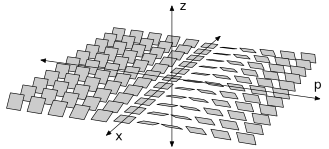
\includegraphics[height=1.5in]{Standard_contact_structure}
		\caption{A visualization of the plane field $\ker \alpha = \spa \left\{ \frac{\partial}{\partial x} + p \frac{\partial}{\partial z}, \frac{\partial}{\partial p}\right\}$.}
		\alttext{A collection of small gray squares at points in the horizontal plane, together with axes labeled $x$, $p$, and $z$. See caption and surrounding text for a mathematical description.}
		\label{fig:contact structure}
	\end{figure}
	
	Solutions to differential equations of the form $F(x,z,z')=0$ produce curves in $(x,z,p)$-space which are everywhere tangent to the plane determined by $\ker \alpha$; these are often called Legendrian curves. This formalism is the basis of an area of mathematics called \emph{contact geometry} or \emph{contact topology}, which has recently been very useful in the study of 3-manifolds, but which historically was developed because of its relevance to thermodynamics and geometric optics; see Geiges's historical survey~\cite{geigesBriefHistoryContact2001} for an introduction to this area.
\end{example}

The plane field described above and illustrated in \Cref{fig:contact structure} is an example of a \emph{distribution}:

\begin{definition}\label{def:distribution}
	A $d$-dimensional \emph{distribution} on a manifold $M$ is a smooth choice of $d$-dimensional subspace $\mathcal{D}(p) \subset T_pM$ for each $p \in M$. Equivalently, $\mathcal{D}$ is a sub-bundle of the tangent bundle $TM$. This means that at each point $p \in M$, there exists a neighborhood $U$ of $p$ and vector fields $X_1, \dots , X_d$ so that $\mathcal{D}(p) = \spa \{X_1(q), \dots , X_d(q)\}$ for any $q \in U$.
	
	A vector field $X \in \mathfrak{X}(M)$ lies in $\mathcal{D}$ if $X(p) \in \mathcal{D}(p)$ for all $p \in M$; by slight abuse of notation, we denote this as $X \in \mathcal{D}$. The distribution is \emph{involutive} if $[X,Y] \in \mathcal{D}$ for all $X,Y \in \mathcal{D}$.
\end{definition}

\begin{example}
	Let $\mathcal{D} = \spa\left\{ \frac{\partial}{\partial x_{i_1}}, \dots , \frac{\partial}{\partial x_{i_k}}\right\}$ for some $1 \leq i_1 < \dots < i_k \leq n$. Then $\mathcal{D}$ is a $k$-dimensional distribution on $\R^n$. Moreover, for any $1 \leq r , \leq k$, 
	\[
		\left[\frac{\partial}{\partial x_{i_r}}, \frac{\partial}{\partial x_{i_s}}\right] = \frac{\partial^2}{\partial x_{i_r}\partial x_{i_s}} - \frac{\partial^2}{\partial x_{i_s}\partial x_{i_r}}  =0
	\]
	since mixed partials commute, so $\mathcal{D}$ is involutive.
\end{example}

\begin{example}\label{ex:standard contact structure involutive}
	Let $\xi = \spa \left\{ \frac{\partial}{\partial x} + p \frac{\partial }{\partial z}, \frac{\partial}{\partial p} \right\} = \ker (dz - p\, dx)$ be the 2-dimensional distribution on $\R^3$ from \Cref{ex:standard contact structure}. Then for any $f \in C^\infty(\R^3)$,
	\begin{align*}
		\left[ \frac{\partial}{\partial x} + p \frac{\partial }{\partial z}, \frac{\partial}{\partial p}\right](f) & = \left(\frac{\partial}{\partial x} + p \frac{\partial }{\partial z}\right)\left(\frac{\partial f}{\partial p}\right) - \frac{\partial}{\partial p} \left(\frac{\partial f}{\partial x} + p \frac{\partial f}{\partial z}\right) \\
		& = \frac{\partial^2 f}{\partial x \partial p} + p \frac{\partial^2 f}{\partial z \partial p} - \frac{\partial^2 f}{\partial p \partial x} - \frac{\partial f}{\partial z} - p\frac{\partial^2 f}{\partial p \partial z} \\
		& = -\frac{\partial f}{\partial z},
	\end{align*}
	so $\left[ \frac{\partial}{\partial x} + p \frac{\partial }{\partial z}, \frac{\partial}{\partial p}\right] = -\frac{\partial}{\partial z} \notin \xi$, so $\xi$ is not involutive. $\xi$ is called the \emph{standard constact structure} on $\R^3$.
\end{example}

\begin{example}\label{ex:S^3 standard contact structure}
	Recall the left-invariant vector fields $X,Y,Z$ on $S^3$ from \Cref{sec:S^3 example}. Let $\zeta = \spa \{Y,Z\} = \ker \alpha$, where $\alpha$ is the 1-form dual to $X$. $\zeta$ is a 2-dimensional distribution on $S^3$. We saw in \Cref{sec:S^3 example} that $[Y,Z] = 2X \notin \zeta$, so $\zeta$ is also not involutive. $\zeta$ is called the \emph{standard tight contact structure} on $S^3$.
\end{example}

\begin{definition}\label{def:integral manifold}
	The image of a smooth embedding $i \from N \to M$ is an \emph{integral manifold} of a distribution $\mathcal{D}$ on $M$ if $(di)_p\left(T_pN\right) = \mathcal{D}(i(p))$ for all $p \in N$. In other words, $N$ has the same dimension as $\mathcal{D}$ and $i(N)$ is everywhere tangent to $\mathcal{D}$.
\end{definition}

\begin{example}
	Consider $\mathcal{D} = \spa \left\{ -y \frac{\partial}{\partial x} + x \frac{\partial}{\partial y}, -z \frac{\partial}{\partial x} + x \frac{\partial}{\partial z}\right\}$ on $\R^3 - \{\vec{0}\}$. Notice, first of all, that $\mathcal{D}$ is involutive since
	\begin{multline*}
		\left[ -y \frac{\partial}{\partial x} + x \frac{\partial}{\partial y}, -z \frac{\partial}{\partial x} + x \frac{\partial}{\partial z}\right] = \left( -y \frac{\partial}{\partial x} + x \frac{\partial}{\partial y}\right) \left( -z \frac{\partial}{\partial x} + x \frac{\partial}{\partial z}\right) - \left( -z \frac{\partial}{\partial x} + x \frac{\partial}{\partial z}\right)\left( -y \frac{\partial}{\partial x} + x \frac{\partial}{\partial y}\right)  \\
		= yz \frac{\partial^2}{\partial x^2} -xz \frac{\partial^2}{\partial y \partial x} -y \frac{\partial}{\partial z} - xy \frac{\partial^2}{\partial x \partial z} + x^2 \frac{\partial^2}{\partial y \partial z} -yz \frac{\partial^2}{\partial x^2} +z \frac{\partial}{\partial y} + xz \frac{\partial^2}{\partial x \partial y} + xy \frac{\partial^2}{\partial z \partial x} -x^2 \frac{\partial^2}{\partial z \partial y} \\
		= -y\frac{\partial }{\partial z} + z \frac{\partial }{\partial y} = - \frac{y}{x} \left(-z \frac{\partial}{\partial x} + x \frac{\partial }{\partial z } \right) + \frac{z}{x} \left( - y \frac{\partial }{\partial x} + x \frac{\partial }{\partial y}\right)  \in \mathcal{D}.
	\end{multline*}
	
	Also, since the cross product
	\[
		\left( -y \frac{\partial}{\partial x} + x \frac{\partial}{\partial y}\right) \times \left( -z \frac{\partial}{\partial x} + x \frac{\partial}{\partial z}\right) = x\left( x \frac{\partial}{\partial x} + y \frac{\partial}{\partial y} +z \frac{\partial}{\partial z} \right)
	\]
	is parallel to the radial field $x \frac{\partial}{\partial x} + y \frac{\partial}{\partial y} +z \frac{\partial}{\partial z}$, we see that $\mathcal{D}$ is everywhere tangent to the concentric spheres centered at the origin, which are integral manifolds for $\mathcal{D}$.
\end{example}

The algebraic condition of involutivity is closely related to the geometric condition of having an integral manifold:

\begin{proposition}\label{prop:integra implies involutive}
	If $\mathcal{D}$ is a smooth distribution on $M$ so that at each $p \in M$ there is an integral manifold of $\mathcal{D}$ passing through $p$, then $\mathcal{D}$ is involutive.
\end{proposition}

\begin{proof}
	If $X,Y \in \mathcal{D}$, then at each $q = i(p) \in i(N)$, we have that $X(q) = (di)_p \widetilde{X}(p)$ and $Y(q) = (di)_p \widetilde{Y}(p)$ for some $\widetilde{X}, \widetilde{Y} \in \mathfrak{X}(N)$. Since $[\widetilde{X}, \widetilde{Y}](p) \in T_pN$, we see that
	\[
		[X,Y](q) = [(di)_p \widetilde{X}(p),(di)_p \widetilde{Y}(p)](i(p)) = (di)_p [\widetilde{X},\widetilde{Y}] \in (di)_p(T_pN) = \mathcal{D}(q)
	\]
	using \Cref{lem:differential of bracket}. So $\mathcal{D}$ is involutive.
\end{proof}

The much more amazing fact is that the converse is true, so we can determine existence integral manifolds by checking involutivity. This is the content of:

\begin{theorem}[Frobenius Theorem]\label{thm:Frobenius}
	Let $\mathcal{D}$ be a $k$-dimensional involutive distribution on a manifold $M$. Then for each $p \in M$ there is an integral manifold of $\mathcal{D}$ passing through $p$.
\end{theorem}

The idea behind the theorem is the following: suppose $\mathcal{D}$ is (locally) spanned by the vector fields $V_1, \dots , V_k$. Remember that the $V_i$ are really first-order differential operators on $M$, so the set $\{V_1, \dots , V_k\}$ determines a first-order homogeneous system of PDEs
\[
	V_1 u = 0 , \dots , V_k u = 0.
\]
If $u \from M \to \R$ is a solution to this system of PDEs, then the level sets of $u$ are tangent to $\spa \{V_1, \dots , V_k\}$. Frobenius' original question was: when are there solutions $u_1, \dots , u_{n-k}$ so that the gradients $\nabla u_1, \dots , \nabla u_{n-k}$ are linearly independent? (There certainly can't be more than $n-k$ solutions, since the gradients will be normal to the level sets and the orthogonal complement of $\spa \{V_1, \dots , V_k\}$ is $(n-k)$-dimensional.)

When there exist such $u_1, \dots , u_{n-k}$, then the level sets of the product map $(u_1, \dots , u_{n-k}) \from M \to \R^{n-k}$ will necessarily be integral manifolds of $\mathcal{D}$.

\begin{proof}[Proof of \Cref{thm:Frobenius}]
	I want to show that, for all $p \in M$, there exists a coordinate chart $(U,\phi)$ so that:
	\begin{enumerate}
		\item $\vec{0} \in U \subset \R^n$
		\item $\phi(\vec{0})=p$
		\item For $\vec{a} = (a_1, \dots , a_n) \in U$, the set $\{q \in M : \phi^{-1}(q)_{k+1} = a_{k+1}, \dots , \phi^{-1}(q)_n = a_n\}$ is an integral manifold of $\mathcal{D}$.
	\end{enumerate}
	
	Since this is a local argument, we may as well assume $M \subset \R^n$ is an open set, $p = \vec{0}$, and, after rotation, $\mathcal{D}(p) = \mathcal{D}(\vec{0}) = \spa \left\{ \frac{\partial}{\partial x_1} , \dots , \frac{\partial}{\partial x_k}\right\}$ is the $k$-plane spanned by the first $k$ coordinate directions.
	
	Let $\pi \from \R^n \to \R^k$ be projection onto the first $k$ coordinates, so that $\left. (d\pi)_{\vec{0}}\right|_{\mathcal{D}} \from \mathcal{D}(\vec{0}) \to T_{\vec{0}} \R^k \cong \R^k$ is an isomorphism, and hence $\left. d\pi\right|_{\mathcal{D}}$ is injective on some neighborhood $U$ of $\vec{0}$.
	
	Therefore, in $U$ there exist unique $V_1, \dots , V_k \in \mathcal{D}$ so that $(d\pi)_q V_i = \left. \frac{\partial}{\partial x_i} \right|_{\pi(q)}$ for all $q \in U$ and for all $i \in \{1 , \dots , k\}$.
	
	Since $\mathcal{D}$ is involutive, $[V_i, V_j ] \in \mathcal{D}$ for all $1 \leq i, j \leq k$. On the other hand,
	\[
		d\pi[V_i,V_j] = [d\pi V_i, d\pi V_j] = \left[\frac{\partial}{\partial x_i}, \frac{\partial}{\partial x_j}\right] = 0,
	\]
	so $[V_i,V_j]= 0$ since $d\pi$ is an isomorphism.
	
	But then we can find local coordinates $y_1, \dots , y_n$ so that $V_i = \frac{\partial}{\partial y_i}$ on $U$ and the sets
	\[
		\{y \in U : y_{k+1} = a_{k+1}, \dots , y_n = a_n \}
	\]
	are integral manifolds of $\mathcal{D}$.
\end{proof}

\begin{example}\label{ex:rotation field distribution}
	Let $M = \R^2 - \{\vec{0}\}$, let $X(u,v) = -v \frac{\partial}{\partial x} + u \frac{\partial}{\partial y}$, and let $\mathcal{D} = \spa \{X\}$. $\mathcal{D}$ is certainly involutive since $[X,X]=0$ by anticommutativity of the Lie bracket, so there must be (local) integral manifolds through each point in $M$. Of course, this example is easy: the integral manifolds are just concentric circles, as we see in \Cref{fig:concentric circles}.
	
	\begin{figure}[htbp]
		\centering
			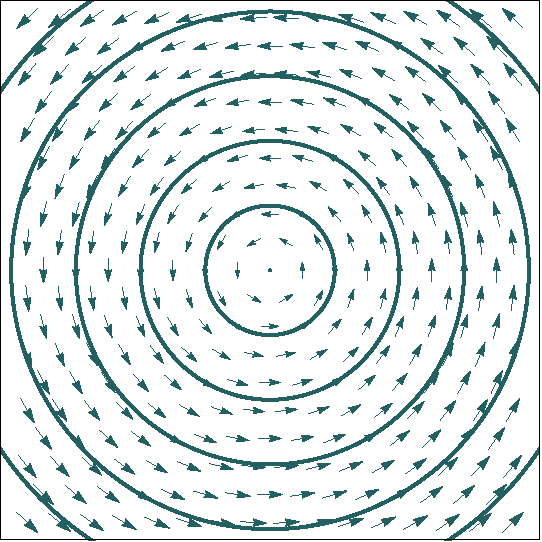
\includegraphics[height=2in]{rotationfield}
		\caption{The vector field $X(u,v) = -v \frac{\partial}{\partial x} + u \frac{\partial}{\partial y}$ together with some integral curves, which are concentric circles.}
		\alttext{The vector field $X$ described in the main text and the caption, depicted by small green arrows, together with some concentric circles of the same color, which are everywhere tangent to the vector field.}
		\label{fig:concentric circles}
	\end{figure}
\end{example}

In fact, anticommutativity of the Lie bracket implies that \emph{all} one-dimensional distributions are involutive, and hence integrable. Said another way: given any line field on a manifold and any point in the manifold, there is a curve passing through the point whose velocity vectors are everywhere tangent to the line field.

\begin{example}
	Consider the standard contact structure $\xi = \spa \left\{ \frac{\partial}{\partial x} + p \frac{\partial}{\partial z}, \frac{\partial}{\partial p} \right\} = \ker(dz - p\, dx)$ on $\R^3$ defined in \Cref{ex:standard contact structure}. We saw in \Cref{ex:standard contact structure involutive} that $\xi$ is not involutive, so there are no surfaces in $\R^3$ which are tangent to $\xi$ in a neighborhood of any point. In other words, $\xi$ is a \emph{totally non-integrable plane field}, which is typically how contact structures on 3-manifolds are defined.
\end{example}

The Frobenius theorem we've proved is a local result (after all, there's no guarantee that the integral manifold we get has diameter $> \epsilon$), but it turns out that the local pieces glue together nicely:

\begin{theorem}[Global Frobenius Theorem]\label{thm:global Frobenius}
	Let $\mathcal{D}$ be an involutive distribution on $M$. Then $M$ is \emph{foliated} by a (disconnected) integral manifold for $\mathcal{D}$. The components of this foliation are called the \emph{maximal integral manifolds} for $\mathcal{D}$.
\end{theorem}

\begin{example}
	The foliation of $\R^2 - \{\vec{0}\}$ corresponding to the distribution $\mathcal{D} = \spa\left\{-y \frac{\partial}{\partial x} + x \frac{\partial}{\partial y}\right\}$ from \Cref{ex:rotation field distribution} is precisely the disjoint union of concentric circles shown in \Cref{fig:circs}.
\end{example}

\begin{figure}[htbp]
	\centering
		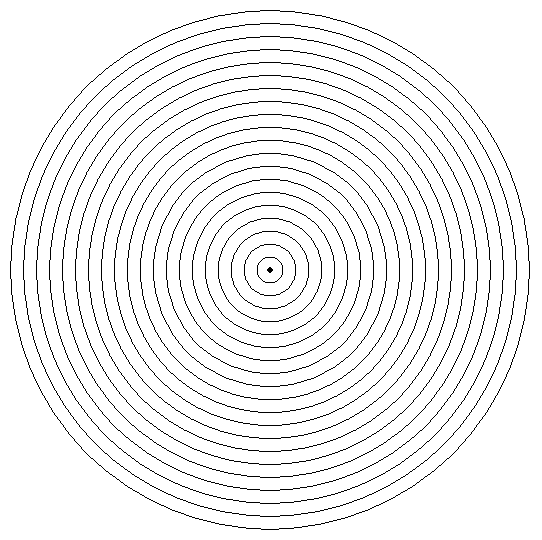
\includegraphics[height=1.2in]{circs}
	\caption{A foliation of the punctured plane by concentric circles.}
	\alttext{Twenty thin concentric circles centered at a point.}
	\label{fig:circs}
\end{figure}

\begin{example}
	The foliation of $\R^3$ corresponding to the involutive distribution $\mathcal{D} = \spa \left\{ \frac{\partial}{\partial x}, \frac{\partial}{\partial y} \right\}$ is the collection of planes parallel to the $xy$-plane, as shown in \Cref{fig:planes}.
\end{example}

\begin{figure}[htbp]
	\centering
		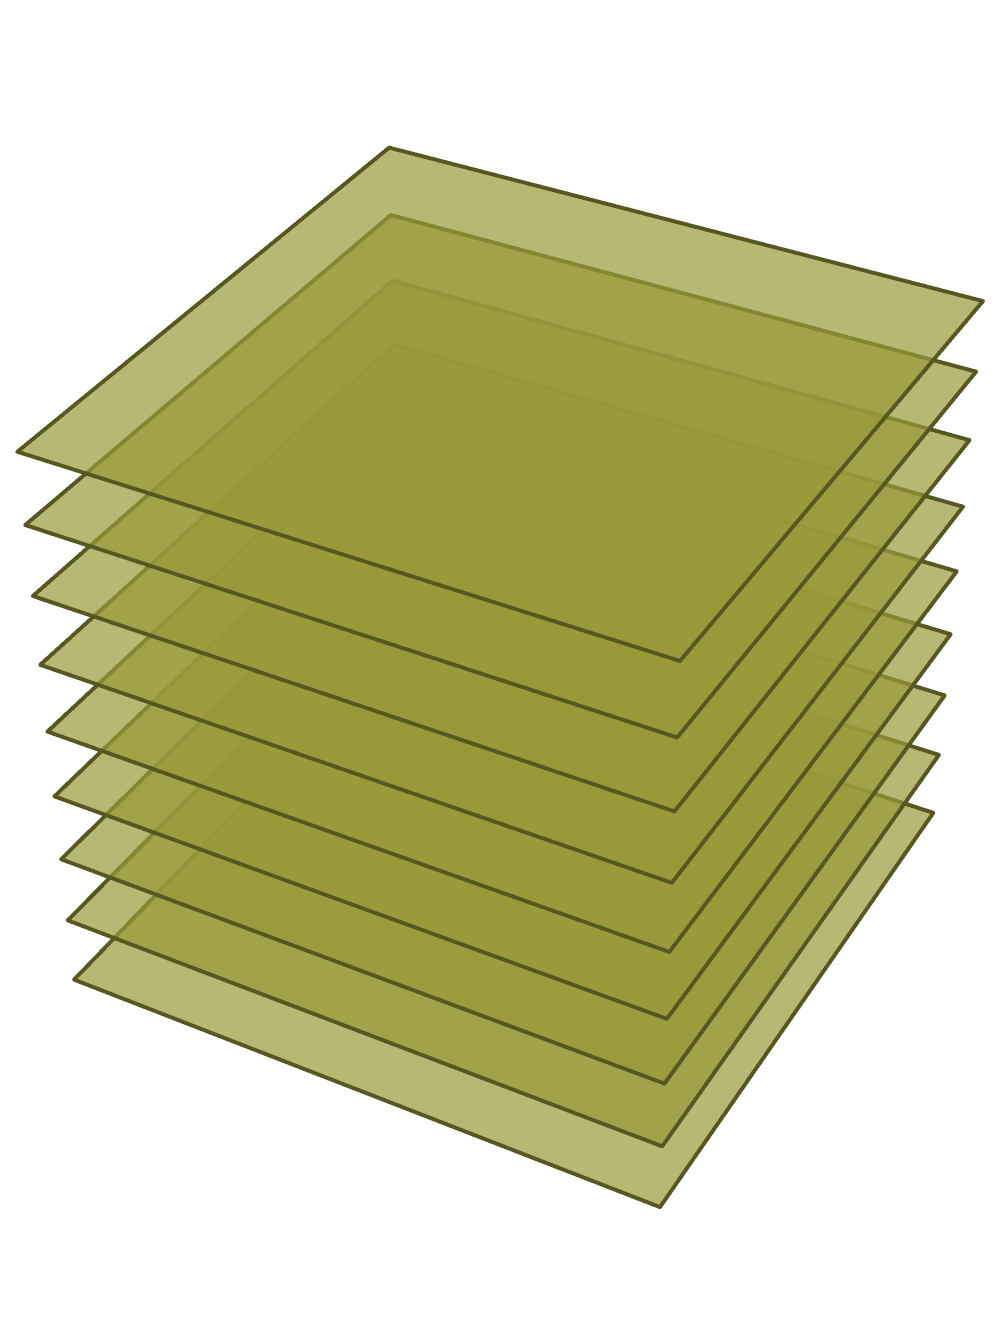
\includegraphics[height=1.8in]{planes}
	\caption{A foliation of $\R^3$ by parallel planes.}
	\alttext{Nine parallel horizontal planes colored green.}
	\label{fig:planes}
\end{figure}